\documentclass[10pt, twocolumn]{article}

\usepackage[letterpaper, portrait, margin=1in]{geometry}
\usepackage{setspace}
\usepackage{graphicx}
\usepackage{float}
\usepackage{geometry}
\usepackage{amsmath}
\usepackage{amssymb}
\usepackage{caption}
\usepackage{multicol}
\usepackage{titlesec}
\usepackage{fontspec}
\usepackage{xpatch}
\usepackage[table]{xcolor}
\usepackage{newfloat}
\usepackage{xltabular}
% \usepackage{multicol}

\usepackage{fancyhdr}
\pagestyle{fancy}
\fancyhf{}
\lhead{\color{gold} \bfseries $\blacktriangleright$ \leftmark}
\rhead{}
\lfoot{Emmanuel College Biology Department}
\rfoot{\thepage}

\definecolor{darkblue}{HTML}{004B87}
\definecolor{gold}{HTML}{F6BE00}
\definecolor{lightblue}{HTML}{00AEEF}

\DeclareFloatingEnvironment[
    name=Instrument,
    placement=H
]{instrument}

\usepackage[backend=biber,style=authoryear]{biblatex}

\usepackage{xparse}% for multiple optional parameters
\usepackage{ifoddpage}% get correct page number

\makeatletter
\let\oldfootcite=\footcite
\RenewDocumentCommand{\footcite}{O{}O{}m}{\checkoddpage
  \@ifundefined{citepage@#3}{}%
  {\ifnum\csname citepage@#3\endcsname<\oddpage@page\relax
      \global\expandafter\let\csname repeatcite@#3\endcsname=\relax
  \fi}%
  \@ifundefined{repeatcite@#3}%
  {\oldfootcite[#1][#2]{#3}%
    \expandafter\xdef\csname repeatcite@#3\endcsname{\thefootnote}%
    \expandafter\xdef\csname citepage@#3\endcsname{\arabic{page}}}%
  {\footnotemark[\csname repeatcite@#3\endcsname]}}
\makeatother

\renewcommand{\headrulewidth}{2pt}
\renewcommand{\headrule}{\hbox to\headwidth{\color{darkblue}\leaders\hrule height \headrulewidth\hfill}}
\renewcommand{\footrulewidth}{2pt}
\renewcommand{\footrule}{\hbox to\headwidth{\color{gold}\leaders\hrule height \headrulewidth\hfill}}

% Some general changes
\DeclareNameAlias{sortname}{last-first}
\renewcommand*{\bibinitdelim}{}
\renewbibmacro*{in:}{%
    \iffieldequalstr{entrytype}{inproceedings}{%
        \printtext{\bibstring{in}\addspace}%
    }{}%
}

% Changes for Book
\csletcs{abx@macro@publisher+location+date@orig}{abx@macro@publisher+location+date}
\renewbibmacro*{publisher+location+date}{%
    \printtext[parens]{\usebibmacro{publisher+location+date@orig}}
}
\DeclareFieldFormat[book]{title}{#1\printunit{\addspace}}

% Changes for inproceedings
\DeclareFieldFormat[inproceedings]{title}{#1\isdot}
\DeclareFieldFormat{booktitle}{#1\addcomma}
\xpatchbibmacro{byeditor+others}{%
    \usebibmacro{byeditor+othersstrg}%
    \setunit{\addspace}%
    \printnames[byeditor]{editor}%
    \clearname{editor}%
}{%
    \printnames[byeditor]{editor}%
    \clearname{editor}
    \addcomma\addspace
    \bibstring{editor}
    \setunit{\addspace}%
}{}{}

% Changes in Article
\DeclareFieldFormat[article]{title}{#1}
\DeclareFieldFormat[article]{journaltitle}{#1\isdot}
\DeclareFieldFormat[article]{volume}{\textit{#1}}
\DeclareFieldFormat[article]{pages}{#1}

\setmainfont{Source Sans 3}

\titleformat{\section}[hang]{\large\bfseries\color{lightblue}}{\thesection}{0.5 em}{}{}

\titleformat{\subsection}[hang]{\normalsize\bfseries\color{lightblue}}{\thesubsection}{0.5 em}{}{}

\titleformat{\subsubsection}[hang]{\normalsize\bfseries\color{gold}}{~}{0.5 em}{}{}


\newcommand{\gitemp}[2] {\samepage{\noindent\textbf{\color{darkblue} $ \blacktriangleright $ {#1}} \\ {#2}} \smallskip}

\newcommand{\gitemn}[2] {\samepage{\noindent\textbf{\color{gray} $ \blacktriangleleft $ {#1}} \\ {#2}} \smallskip} 

\addbibresource{references.bib}

\title{A Review of Inclusive Practices and Language to Advance Scientific Identity of Marginalized Undergraduate Biology Students}
\author{Mickey Barron; Dr. Janel Cabrera, PhD}
\date{Emmanuel College \\ ~ \\ 2021-12-06}

\begin{document}

\begingroup

    \onecolumn

    \maketitle

    \abstract{This paper is an alpha release of resources for use in a student-lead review and think tank.}

    \tableofcontents

    \twocolumn


\endgroup

\section{Introduction}

    This review was developed in order to promote diversity, equity, and inclusion (DEI) within the undergraduate biology and/or science, technology, engineering, and mathematics (STEM) settings. Specifically, this review aims to provide literature and recommendations to advance marginalized students' scientific identity (Sci-ID). Moreover, this review proposes an extension of the definition of Sci-ID drawing from the principles of computational identity (CI).

    \subsection{Scientific identity}

        Scientific identity (Sci-ID) is broadly defined as an identity model of one's inner sense of their alignment with science: whether or not they are a ``science person''.\footcite{salehjee_models_2018} \cite{oseguera_examining_2019} found that Black students had significantly lower Sci-ID than their white counterparts and identified that Sci-ID is a strong predictor of persistnce in science. Moreover, the study found that intervention targeted towards improving Black students' Sci-ID is successful in raising Sci-ID to levels comparable to their white counterparts.\footcite{oseguera_examining_2019}
        
        Sci-ID development, therefore, is important to understand. \cite{salehjee_models_2018} establishes a seven-domain conjugated model of Sci-ID development. Sci-ID is influenced by: (1) global forces, such as one's identity, (2) social agencies and agents, such as educational institutes, teachers, and parents, (3) transformational learning experiences, including accidental and planned events that shapes one's perception of science, (4) one's openness to new information, (5) personal preference that selects for favored learning experiences, (6) individual internal agency, or one's internal drive to develop their Sci-ID, and (7) their core identity, which can be stable or fluid. Domains 1-3 direct information through domains 4-6, which filter what information acts on and develops domain 7, the core Sci-ID.\footcite{salehjee_models_2018}

        Sci-ID's development is well-defined, however, Sci-ID itself varies in definition across literature. Thus, this review proposes a three-part definition drawing upon an analog from computer science: computational identity (CI). \cite{brousseau_position_2019} defines CI as a key factor in students' persistence in the pursuit of computing comprising of three components: (1) the perception that computing is useful, (2) self-efficacy in computing, and (3) a sense of belonging in computing.\footcite{brousseau_position_2019} Using this definition, this paper proposes a generalization of CI to Sci-ID, defining Sci-ID by three analogous components: (1) the perception that science is useful, (2) self-efficacy in science, and (3) a sense of belonging in science.\footcite{brousseau_position_2019} This definition is summarized in figure \ref{fig:sci_id}.

        \begin{figure}[h]
            \rule{\columnwidth}{1pt}
            \begin{center}
            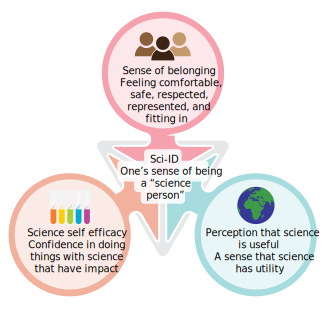
\includegraphics[width = \columnwidth]{figures/sci-id.pdf}
            \end{center}
            \caption{\textbf{Defining scientific identity (Sci-ID): a three-component system.} This diagram summarizes the definition of Sci-ID and its three components: (1) the perception that science is useful, (2) science self efficacy, and (3) a sense of belonging in science.}
            \label{fig:sci_id}
            \rule{\columnwidth}{1pt}
        \end{figure}

        \subsubsection{Perception that science is useful}

            An integral aspect of one's Sci-ID is one's perception that science is useful, in other words, they must have a sense that science is ``worth doing''. Moreover, one must feel that science is functional and applicable to their life. This is important as, per Eccles' expectancy-value theory\footcite{wigfield_expectancyvalue_2000}, the higher a student's subjective task value for science (their perception of the value and utility of learning and doing science), the more motivated they are to persist in science.\footcite{brousseau_position_2019} This perception that science is useful is critical to one's Sci-ID as it directly impacts their motivation and persistence in science.

        \subsubsection{Science self efficacy}

            Science self-efficacy is one's own confidence in their ability to do science.\footcite{ballen_enhancing_2017} To elaborate, it is one's sense that not only can they do science, but in combination with their perception that science is useful, the things they can do with science have utility and impact.\footcite{brousseau_position_2019}  \cite{bandura_perceived_1993} found that one's self efficacy is a strong indicator of one's anxiety, motivation, and performance in a given domain; high self-efficacy conflates with strong performance and motivation with minimized anxiety whereas low self-efficacy is accompanied by high anxiety, a lack of motivation, and poor performance.\footcite{bandura_perceived_1993} Thus, it becomes apparent that science self efficacy is critical to one's Sci-ID; their confidence in science directly impacts their motivation to persist and their performance.

        \subsubsection{Sense of belonging in science}

            \begin{figure*}[t!]
                \begin{center}
                \includegraphics[height = 0.35 \paperheight]{figures/sense_of_belonging.pdf}
                \end{center}
                \caption{\textbf{Model of belonging differs for privileged and marginalized students and is dictated by involvement, relationships, and environment.} This diagram, sourced from \cite{vaccaro_development_2016}, summarizes key components of a sense of belonging and how those differ between privileged and marginalized students across environment, relationships, and involvement. Privileged students are represented in red and marginalized students are represented in blue.}
                \label{fig:sense_of_belonging}
                \rule{\textwidth}{1pt}
            \end{figure*}

            A student's sense of belonging consists of two major components: comfortability and fitting in; these components manifest across three domains: environment, relationships, and involvement. Students feel as though they belong when they feel comfort with others and in their surroundings and that they fit in with others and their surroundings on their campus.\footcite{vaccaro_development_2016}
            
            Developing a sense of belonging differs between marginalized and privileged students. It is important to understand how to support a sense of belonging for both types of students.\footcite{vaccaro_development_2016} Figure \ref{fig:sense_of_belonging} summarizes the key elements of the development of the sense of belonging and how it differs between privileged and marginalized students across the three domains. \cite{vaccaro_development_2016} found key differences emerge when analyzing the sense of belonging for marginalized students. In addition to feeling comfortable and fitting in, marginalized students value safety and respect where they feel physically safe in their settings, welcomed, accepted, and that both themself and their culture are respected.\footcite{vaccaro_development_2016}

            Students' environment impacts their sense of belonging; this impact varies greatly between marginalized and privileged students. Privileged students feel a sense of belonging in environments in which they describe as friendly, fun, and comfortable; these students typically attribute a sense of belonging exclusively to positive descriptors regarding their environment. Marginalized students, however, typically feel a lack of belonging in their environment as a result of feeling like the ``only one'' due to a lack of campus diversity and a restriction of authenticity in their expression due to judgement from peers and unfair treatment. Thus, marginalized students require support in their authentic expression and diverse representation to feel belonging in their environment.\footcite{vaccaro_development_2016}

            Relationships are critical to students' sense of belonging. Privileged students seek a sense of familiarity with others, having fun, and receiving support in tasks in order to feel a sense of belonging. Marginalized students, rather, require deep connection and the ability to be comfortably authentic in their relationships in order to have a sense of belonging. Moreover, marginalized students may actively reject relationships that do not embrace their authentic expression.\footcite{vaccaro_development_2016}

            Involvement, too, is crucial to students' sense of belonging. Again, privileged and marginalized students value different aspects of belonging in involvement. Privileged students value fun and enjoyable involvement and when their involvement has a perceivable impact. Marginalized students, on the other hand, require involvement that allows and encourages authentic expression. Further, marginalized students value involvement that fosters authentic conversations and connections. This sense of authenticity is critical for marginalized students; involvement that did not nurture this authenticity did not foster belonging for these students and often led to these students discontinuing their involvement.\footcite{vaccaro_development_2016}

            % A student's sense of belonging, too, is critical to their Sci-ID, and therefore their performance and persistance in science. It becomes apparent that this sense of belonging must be prioritized and nurtured along with the other aspects of marginalized students' Sci-ID

            Therefore, a marginalized students' sense of belonging is critical to their development and maintenance of Sci-ID, and thus, their performance and persistence in science. Their sense of belonging must be prioritized and nurtured, along with the other aspects of their Sci-ID.

    \subsection{Nurturing scientific identities of marginalized students}
        
        Given the dependence of marginalized students' perserverance and performance in science on scientific identity (Sci-ID), it becomes increasingly apparent that educational institutions must nurture marginalized students' Sci-IDs. For the undergraduate sciences, this paper presents a glossary of diversity, equity, and inclusion (DEI)-oriented terms sourced from recent academic journal articles, domain-specific recommendations, and an index of diverse and accurately-represented scientists to be used by undergraduate professors to nurture the Sci-ID of marginalized students and proposed studies to evaluate the efficacy of these recommendations and resources. 

\section{Methodology}
        
    The recommended intervention provided in this paper --- the glossary, recommendations, and index of diverse and accurately-represented scientists --- is suggested for use to develop the scientific identity based upon reviewed literature. It, however, has not been validated. Thus, this paper provides a proposed study design accompanied by survey instruments to collect student identities, measure scientific identity of students, quantify instructor adherence to guidelines, and calculate a coefficient of relevance representative of the degree to which these guidelines apply to a given course.

    This study design seeks to do the following three items: (1) validate the instruments, (2) describe the current landscape of Sci-ID across students of different identities at Emmanuel College, and (3) evaluate the utility of the recommended intervention in the improvement of student Sci-ID. 

    \subsection{The Measurements and Instruments}

        The instruments to be employed in the proposed study are defined herein. It should be noted that these are named measurements and the instruments that measure them are referred to explicitly as instruments.

        \subsubsection{Quantification of Sci-ID (QoS)}
            The instrument to measure student Sci-ID, or their Quantification of Sci-ID (QoS) is defined in instrument \ref{inst:sci-id}. It calculates a QoS score from 0 - 50, 0 being no Sci-ID, 50 being the most Sci-ID. It measures both the student's perception of their Sci-ID over the three domains and their effective Sci-ID.

        \subsubsection{Qualitative Identity Index (QII)}
            The instrument used to describe a student's identity, their Qualitative Identity Index (QII), is defined in instrument \ref{inst:identity-inv}. Their QII describes the student's comprehensive identities and their effective privileges and power.

        \subsubsection{Instructor Guideline Adherence Rating (IGAR)}
            The instrument used to rate a course's instructor based upon their adherence to the intervention guidelines recommended by this paper, or their Instructor Guideline Adherence Rating (IGAR), is defined in instrument \ref{inst:instructor-adherence}. The IGAR scores instructors from 0 - 10, 0 being no adherence, 10 being consistent and strong adherence based upon both their presentation of information and the resources they provide to students, including textbooks, slides, handouts, and more.
        
        \subsubsection{Course Coefficient of Relevance (CCoR)}
            The instrument used to measure a course's relevance and the applicability of the guidelines recommended in this paper, or the Course Coefficient of Relevance (CCoR), is defined in instrument \ref{inst:relevance-coeff}. It calculates a coefficient from 0 - 1 that describes to what degree and/or what portion of the guidelines apply, 0 being not at all, 1 being completely.
    
    \subsection{Research Questions}

        This study aims to pose research questions accompanied by hypotheses and study designs to achieve the defined goals.      

        \subsubsection{Research Question 1: Are the instruments valid?}

            In order to evaluate student Sci-ID both pre- and post-intervention, the instrument measuring Sci-ID, the QoS instrument, and its supporting instruments measuring environmental variables must all be validated. It is hypothesized that, if the QoS instrument is valid, then the QoS and the students' final grades would have a statistically significant positive correlation. The remaining three instruments measure environmental variables that are suspected to impact Sci-ID. These are the QII, IGAR, and CCoR instruments. It is hypothesized that the IGAR instrument is valid if the IGAR significantly and positively correlates to the students' change in QoS. Continuing, the CCoR instrument is hypothesized to be valid if the variance of student QoS significantly and inversely relates to the CCoR. Finally, the QII instrument is hypothesized to be valid if student QoS varies insignificantly within populations with similar responses.

        \subsubsection{Research Question 2: What is the current landscape of undergraduate STEM student Sci-ID?}

            This portion of the study aims to describe the current Sci-ID of undergraduate students in STEM and how it differs between students of different identities in order to identify populations of students with higher risks of poor performance and low perserverance in STEM using a descriptive study design. Thus, this study will compare QII variables to initial QoS scores to identify any vulnerable populations.

        \subsubsection{Research Question 3: How does the proposed intervention change undergraduate STEM student Sci-ID?}
            
            This portion of the study aims to assess the efficacy of the proposed intervention in improving STEM student Sci-ID both across all students and within underrepresented populations. It shall follow a before-after study design in which student QoS scores are measured before and after the intervention and the change in QoS is analyzed in relation to student QIIs, IGARs, and the CCoRs. It is hypothesized that if the intervention defined in this paper is effective in improving all student's Sci-ID, QoS scores will show a statistically significant positive change. The IGAR and CCoR will be used to assess which components of the intervention are most impactful under the hypothesis that for each component, if that component is effective in developing student Sci-ID, then the component's IGAR and CCoR subscores will have a statistically significant positive correlation to the change in QoS scores. There also will be a descriptive component analyzing the change in QoS scores between students of different identities using the QII.

    \subsection{The Proposed Study Design}

        This study shall follow the design as defined chronologically herein. Within the first 14 days of a 16 week course, the students will be assessed for their QoS and optionally their QII using their respective instruments. After 7 - 9 weeks, the instructor and/or an auditor will evaluate the instructor for their IGAR using the IGAR instrument. Within the last 2 weeks of the course, students will be assessed for their QoS and optionnally their QII using their respective instruments. Instructors will be assessed for their IGAR by the instructors and/or an auditor using the IGAR instrument and the course's CCoR will be calculated by the instructor, study administrators, and/or auditors, using the CCoR isntrument. These measurements will be statistically analyzed as appropriate.

\section{The Glossary}
    
    The glossary was constructed from a review of literature. The glossary lists: \\

    \gitemp{inclusive terms}{ that are suggested for use by individuals that are not part of the community and/or identity being discussed which are denoted with a $\blacktriangleright$ and highlighting them in blue.}

    \gitemn{exclusive terms}{ that are not suggested for use by individuals that are not part of the community and/or identity being discussedthat do not identify with the identity in reference which are denoted with a $\blacktriangleleft$ and highlighting them in gray.}

    \noindent It should be noted that these classifications are based on their use by individuals who are not a part of the community and/or identity being discussed; Ultimately, individuals who identify with the identity and/or community being discussed should be listened to and their self-identified labels and chosen terminology should be used. Self-labelling and chosen terminology is, typically, a result of personal context, intersectionality, self-agency, and, in some cases, a form of resistance.\footcite{wagaman_self-definition_2016} It should be the right of individuals who identify with the identity and/or community to make these choices as it empowers them and centers their needs and autonomy in discussions regarding them. \footcite{botha_does_2021}
    
    Additionally, these classifications make no indication on the moral good or bad of the term they are describing, rather they indicate the general acceptability of using that term to describe the phenomenon.

    Finally, it should be noted that, in this paper, these definitions are categorized under the category of which they are most related to. This method of categorization, however, is not representative of intersectionality of identities. Thus, readers are encouraged to visit the digital glossary at github.com/ec-belonging-in-biology/sci-id-development where each definition is tagged with each of its relevant categories and can be filtered, which better represents the intersectional nature of the terms defined herein.

    \subsection{General}

        \gitemp{accountability}{in the social justice context, an individual and/or group's sense of responsibility as a result of their identity both privileging them at the expense of the marginalization of a group and providing them agency to use their privilege to align with and support the marginalized group.\footcite{wooldridge_what_2019}} \\
        \gitemp{ally}{an advocate or supporter of marginalized groups who have a reasonable understanding of the inequities and discrimination marginalized groups face and recognize their part in perpetuating the status quo that ultimately oppresses these groups. \footcite{nash_male_2021}} \\
        \gitemp{assimilation}{the process in which the dominant culture absorbs individuals from a minority population, while stripping their culture and norms away from them under the precedent that the dominant culture believes the minority culture is in one or more ways inferior to them. \footcite{ramirez_assimilation_2020}} \\
        \gitemp{bigot}{one with an aggressive intolerance that actively oppresses members of other identities while upholding a seemingly indestructible glorification of their own viewpoints and identity. \footcite{corvino_puzzles_2019}} \\
        \gitemp{biological essentialism}{the weaponization of biological sciences in which claims of superiority or absolute right and wrong are made on the basis of a crude and over-simplified or ``essential'' concept. \footcite{greene_biological_2020}} \\
        \gitemp{collective accountability}{the collective action taken by a privileged group to hold themselves accountable in dismantling large-scale oppressive systems.\footcite{wooldridge_what_2019}} \\
        \gitemp{cultural appropriation}{the act of individuals who do not identify as part of a culture stealing expressions, artifacts, intellectual property, history, and ways of knowledge from said culture without permission. \footcite{howard_equity_2020} This can manifest itself in one of at least three forms: subject, content, and tangible object appropriation.\footcite{lalonde_does_2021}} \\
        \gitemp{cultural content appropriation}{the use of a culture's property as a part of a cultural outsider's work, such as a white Internet influencer's use of African American Vernacular English in their content. \footcite{lalonde_does_2021}} \\
        \gitemp{cultural subject appropriation}{the representation of a culture by someone who is not part of that culture, such as a non-Indigenous person making a documentary on Indigenous peoples. \footcite{lalonde_does_2021}} \\
        \gitemp{cultural tangible object appropriation}{the stealing of culturally-significant artifacts, human remains, and/or destruction of culturally-significant landmarks,\footcite{lalonde_does_2021} such as the desecration of the Black Hills, sacred to the Lakota Sioux, into Mount Rushmore.\footcite{cottrell_mind_2020}} \\
        \gitemp{culture}{a learned and dynamic social and individual construct that is a descriptive part of one's identity that manifests at several different depths, affects one's social and biological behavior and interpretations and perceptions of others' behaviors, ranges in applicability from individual to global used to associate with a social group. Individuals who identify as a part of a culture may vary in their degree of association and which aspects of a culture they specifically associate with.\footcite{spencer-oatey_what_2012}} \\
        \gitemp{distal stressors}{stresses exerted by external prejudiced events on a marginalized person as a result of one or more of their identities. \footcite{lindley_gender_2020}} \\
        \gitemp{diversity}{the heterogeneity, in other words, the sense of individual uniqueness, of people as a result of each person's individual ideologies, identities and lived experiences.\footcite{kvam_defining_2018}} \\
        \gitemp{equality}{the ideal that every individual receives the same amount of resources and opportunities.\footcite{buchholtz_equity_2020}} \\
        \gitemp{equity}{the ideal that every individual is allocated a variable amount of resources and opportunities to (1) counterbalance any disadvantage not resulting from an individual's choice and (2) to reward or punish in proportion to an individual's contribution to an impact or outcome.\footcite{buchholtz_equity_2020}} \\
        \gitemp{identity-first language}{the language pattern that lists the one's identity and then the subject, the person or other descriptor, such as Black man, or disabled person. \footcite{bogart_ableism_2019}} \\
        \gitemp{implicit bias}{associations made outside one's conscious awareness that result in negative attitudes towards individuals based upon stereotyped characteristics of a certain identity. \footcite{fitzgerald_implicit_2017}} \\
        \gitemp{inclusion}{the genuine empowerment of previously excluded communities and identities so that they may make meaningful contributions in decision making, be respected as their authentic self, and treated equitably. \footcite{shore_inclusive_2018}} \\
        \gitemp{intersectionality}{a framework to approach the evaluation of an individual that not only recognizes one's multiple identities, but understands that their identities are interconnected and interdependent on both the personal, community, and sociostructurally levels. \footcite{atewologun_intersectionality_2018}} \\
        \gitemp{marginalization}{the act of a society deplatforming and pushing people away from economic, sociopolitical, and cultural participation on the basis of identity, lived experience, and/or ideology that ultimately results in a maintained power imbalance between the dominating and marginalized identities and leads to deterioration of marginalized persons. \footcite{alakhunova_defining_2015}} \\
        \gitemp{minority stress model}{a perspective that distress experienced by marginalized individuals regarding their identity(ies) is not solely a result of external (distal) prejudiced events, but also internalized (proximal) stressors experienced both directly and indirectly as a result of existing in a prejudiced society. \footcite{lindley_gender_2020}} \\
        \gitemp{multicultural awareness}{a component of multicultural competence that consists of essential attitudes, biases, assumptions, and values that both consciously and unconsciously shape one's world view. \footcite{pope_multicultural_2019}} \\
        \gitemp{multicultural competence}{a three-component system of authentic understanding of other cultures that consists of multicultural awareness, knowledge, and skills. \footcite{pope_multicultural_2019}} \\
        \gitemp{multicultural knowledge}{a component of multicultural competence that consists of the body of knowledge one has regarding other cultures. \footcite{pope_multicultural_2019}} \\
        \gitemp{multicultural skills}{a component of multicultural competence that describes the ability of one to apply their multicultural awareness and knowledge to their daily interactions, activities, and thoughts.  \footcite{pope_multicultural_2019}} \\
        \gitemp{oppression}{the process in which two populations become inequal as a result of one harming the other for their own benefit systematically and systemically through the behaviors of stereotyping, prejudice, and discrimination or the state in which a dominant population uses their power to exploit, marginalize, exert violence on, and inferiorize the harmed population. \footcite{david_psychology_2017}} \\
        \gitemp{personal accountability}{the actions taken by an individual to hold themselves accountable in advancing a collective approach towards transforming higher oppressive systems. While this is important, personal accountability should not be the focus of accountability as it undermines accountability's emphasis of collective action.\footcite{wooldridge_what_2019}} \\
        \gitemp{person-first language}{the language pattern that lists the subject, the person or other descriptor, followed by the identity, such as student with disabilities or member of the gay community. \footcite{bogart_ableism_2019}} \\
        \gitemp{power}{the ability to influence others' thoughts, actions, well-beings, and emotions that can be obtained through several routes or combinations of routes, one commonly being control over valuable resources. \footcite{ten_brinke_theories_2020}} \\
        \gitemp{prejudice}{a sentiment of devalument towards another group coupled with the glorification of another resulting in a differential and selective behavior typically reinforced by stereotypes. \footcite{bergh_mapping_2021}} \\
        \gitemp{privilege}{one's advantage resultant of their membership in a group or alignment with an identity in contexts where that membership and/or alignment should not have an effect. \footcite{lowe_privilege_2020}} \\
        \gitemp{proximal stressors}{stresses exerted by an internal force on a marginalized person as a result of one or more of their identities. \footcite{lindley_gender_2020}} \\
        \gitemp{reparations}{resources and/or time given to those who have collectively or individually suffered any mental and/or physical loss and/or damage by the responsible group delivered to alleviate the harm done. \footcite{moffett_transitional_2016}} \\
        \gitemp{restorative justice}{a framework to respond to crimes and other harm done to an individual or community that prioritizes the restoration of the harmed party by the responsible party to a state reasonably similar to the state of the harmed party prior to the incident} \\
        \gitemp{social justice}{the call to act in ways that advance societies towards ones in which resources are distributed equitably and all members a physically and psychologically safe and secure. \footcite{pope_multicultural_2019}} \\
        \gitemp{stereotype}{an attitude established by society that associates certain behaviors and traits with members of a particular social group to a stronger degree than members of other social groups, even if inaccurate. \footcite{puddifoot_how_2021}} \\
        \gitemp{tokenism}{the act of symbolic, ingenuine, or otherwise performative efforts to appear to promote diversity, equity, and inclusion while maintaining oppressive systems and practices that are of benefit. \footcite{hahn_tokenism_2017}} \\
    
    
    \subsection{Race \& Ethnicity}    

        \gitemp{ethnicity}{an identity predominantly identified by a perceived common ancestry, culture, and/or history.\footcite{clair_racism_2015}} \\
        \gitemp{race}{generally understood as a completely social construct with no biological basis, it is the perceived patterns of physical differences used to differentiate groups of people.\footcite{clair_racism_2015}} \\
    

        \subsubsection{Race}

            \gitemp{anti-Black}{an ideology comprised of stereotypes, beliefs, assumptions, and connotations of Black people based on a perceived difference that simultaneously compels the discrimination and systemic marginalization\footcite{nighaoui_color_2017} of Black people while also disregarding Black institutions and policies.\footcite{noauthor_racial_nodate}} \\
            \gitemp{anti-racism}{the recognition of racism and understanding of critical race theory that centers the experiences of people of color to actively challenge and oppose the roles of racism in structures, practices, and discourses. \footcite{alderman_reflections_2021}} \\
            \gitemp{anti-racist}{one who actively opposes the roles of racism in structures, practices, and discourses by centering the experiences of people of color and understanding the depth and scope of racism and critical race theory. \footcite{alderman_reflections_2021}} \\
            \gitemp{BIPOC}{an initialism for Black, Indigenous, and People of Color coined with the intent to acknowledge the struggles Black and Indigenous populations face and have faced in America \footcite{titanji_diverse_2020} used to describe people who are not white racially, ethnically, or nationally. \footcite{perez_diversitys_2021}} \\
            \gitemp{Black Lives Matter}{founded in 2013 and often abbreviated as the initialism BLM, it is a movement in response to the acquittal of Trayvon Martin's murderer that seeks to dismantle white supremacy and restore power to Black Americans while creating space for Black imagination, innovation, and Black joy. \footcite{bell_making_2020}} \\
            \gitemp{covert racism}{also known as implicit racism, it is an instance of racism where unconsciously triggered beliefs of inferiority, negative attitudes towards, or assumptions of another race causes acts of racial discrimination.\footcite{clair_racism_2015}} \\
            \gitemp{Critical Race Theory}{typically abbreviated to the initialism CRT, it is a synthesis of thematic challenging of the status-quo understanding of race and its implications in society. \footcite{bracey_toward_2015}} \\
            \gitemp{cultural racism}{suggested as, perhaps, a more accurate descriptor of modern day `racism', it is the absolutization of ethno-cultural origin used to discriminate, marginalize, segregate, exile, or otherwise exclude. \footcite{rodat_cultural_2017}} \\
            \gitemp{diaspora}{an international identity and community of those that live outside of their homeland either due to voluntary or involuntary movement with a strong sense of cohesive community and group identity that maintains strong material and symbolic ties with their homeland. \footcite{grossman_toward_2019}} \\
            \gitemp{indigeneity}{the attribute of the Indigenous identity that acknowledges the inextricable relationship of a population and the land(s) on which they live or their ancestors lived whom, typically, have persisted through some form of colonialism. \footcite{bello-bravo_when_2019}} \\
            \gitemp{Indigenous}{a complex racial and ethnic identity uniquely characterized by its attribute of indigeneity that represents populations that established themselves on a certain region of land and, for the majority of them, persisted through some form of colonialism. \footcite{bello-bravo_when_2019}} \\
            \gitemp{individual racism}{an individual's prejudices, stereotypes, and attitudes towards a race and associated discrimination and actions. \footcite{salter_racism_2018}} \\
            \gitemp{institutional racism}{while it can be overt, it is a typically covert form of racism that results from racist policies, systems, and general norms in an institution or system that discriminate against and/or exploit certain races.\footcite{clair_racism_2015}} \\
            \gitemp{model minority}{an idealized and stereotyped portrayal of Asian Americans that renders their continued struggles invisible and highlights socioeconomic success and obedience after overcoming past oppression and hardships attempting to reinforce the illusion that racism is a problem of the past in the United States. \footcite{shih_impacts_2019}} \\
            \gitemp{overt racism}{also known as explicit racism, an instance of racism where racist ideas are blatantly clear, for example, the use of racial slurs.\footcite{mosley_critical_2021}} \\
            \gitemp{People of Color}{often abbreviated as the initialism PoC or POC, People of Color denotes those that are not white racially, ethnically, or nationally. \footcite{perez_diversitys_2021}} \\
            \gitemp{Racial Identity Development Theory}{a model used to describe how the external factors of society shape and develop one's internal perception of their racial identity that evaluates several external forces and their roles in racial identity development. \footcite{wijeyesinghe_new_2012}} \\
            \gitemp{racial trauma}{also referred to as race-based traumatic stress, it is the collective psychological, emotional, and physical chronic injury as a result of experiencing racism, including overt, covert, interpersonal, institutional, and systemic racism.\footcite{mosley_critical_2021}} \\
            \gitemp{racism}{distinctly different from racial discrimination and inequality, it is an ideology of racial domination in which presumed cultural and/or biological superiority is used to prescribe, justify, or incite inferior treatment of another racial group. \footcite{clair_racism_2015}} \\
            \gitemp{white fragility}{an often weaponized phenomenon deeply rooted in entitlement and superiority in which white people exhibit an aversion to, aggression towards, and/or become defensive in response to discomfort and/or anxiety from an acknowledgement of their own individual role as a white person in racism. \footcite{diangelo_white_2018}} \\
            \gitemp{white privilege}{the socioeconomic, political, cultural, and psychological advantages of whiteness often weaponized in the oppression of people of color. \footcite{blacksher_white_2021}} \\
            \gitemp{white supremacy}{the racial international power system that centers white racial supremacy and its related practices that acts through many social and political relationships to unequally distribute power to white people while deplatforming members of other races. \footcite{beliso-de_jesus_special_2019}} \\

        \subsubsection{Ethnicity}

            \gitemp{ethnocentrism}{a universal phenomenon, equally cognitive, affective, evaluative, and normative, in which, within a society, there is an implied distinction between the one's ethnicity and others' that centers one's ethnicity resulting in claims of superiority, attitudes of pride and vanity towards one's ethnicity, and despise for others'. \footcite{rodat_cultural_2017}} \\
            \gitemp{xenophobia}{negative pessimistic views against either particular or all ethnic groups other than one's ethnic group typically on the basis of prevention of cultural and ethnic mixing between two or more populations due to ``self-preference'' of one's own group. \footcite{rodat_cultural_2017} and used to describe anti-immigrant attitudes that pose aggressive prejudices to those migrating to other countries. \footcite{suleman_xenophobia_2018}} \\
        

    \subsection{Sex \& Gender}

        \gitemp{gender binary}{the purely sociocultural construct, with no basis in biological science, of sex and gender existing as two discrete options, male and female. \footcite{hyde_future_2018}} \\
        \gitemp{two-spirit}{an identifier used by indigenous peoples  to describe a robust and diverse range of identities pertaining to sex, gender, and sexuality that provides is unique and exclusive to indigenous communities to provide a buffer from western assimilation. \footcite{robinson_two_2020}} \\
            

        \subsubsection{Gender}

            \gitemp{androgyny}{a gender expression modality that can be understood as the co-presence of, integration of, and/or transcendence beyond masculinity and femininity. \footcite{galupo_having_2021}} \\
            \gitemp{bigender}{a descriptor of someone who switch between two fixed genders or experience a combination of both identities simultaneously. \footcite{thorne_terminology_2019}} \\
            \gitemp{binding}{a technique used to de-accentuate the breasts in order to help align one's physical appearance with their gender. \footcite{rood_identity_2017}} \\
            \gitemp{bottom surgery}{gender affirming surgery in which the genitals are reconstructed such that they align with one's gender, such as a vaginoplasty, phalloplasty, metoidioplasty, and others. \footcite{puckett_barriers_2018}} \\
            \gitemp{cisgender}{a descriptor of those who self-identify with the gender assigned to them at birth.  \footcite{fiani_navigating_2018}} \\
            \gitemp{femininity}{a gender expression modality typically associated with those that are female and is characterized by people-oriented behavior, nurturing nature, and empathy.  \footcite{parent_inductive_2020}} \\
            \gitemp{gender}{the intersection of social and personal influences and one's internal experiences that guides one's alignment (or lack thereof) with one or more gendered sociocultural archetypes (e.g. nonbinary, female, male, genderqueer) \footcite{fiani_navigating_2018}} \\
            \gitemp{gender dysphoria}{a broad descriptor, ranging in concept from a diagnosis to a feeling, that is distress and/or discomfort experienced as a result of malalignment of one's sex assigned at birth with their gender. \footcite{lindley_gender_2020}} \\
            \gitemp{gender euphoria}{powerfully positive experiences characterized by distinct satisfaction and/or joy as a result of one's gender corresponding with their sex characteristics. \footcite{beischel_little_2021}} \\
            \gitemp{gender expression}{one's external representation of their gender through dress, demeanor, behavior, and/or other factors, typically along axes of masculinity, femininity, both, or neither. \footcite{sweeney_influence_2015}} \\
            \gitemp{gender-affirming care}{a category of medical treatments and procedures that help mitigate feelings of gender dysphoria. \footcite{puckett_barriers_2018}} \\
            \gitemp{genderqueer}{a descriptor of someone whose gender lies outside of or in no relation to the gender binary. \footcite{thorne_terminology_2019}} \\
            \gitemp{hormone therapy}{gender-affirming care that aligns one's hormone levels with that of their gender. \footcite{puckett_barriers_2018}} \\
            \gitemp{masculinity}{a gender expression modality typically associated with those that are male and is characterized by being tall, being strong, having body and facial hair, having a deeper voice, with interests in sports and physical fitness. \footcite{parent_inductive_2020}} \\
            \gitemp{nonbinary}{a descriptor of someone whose gender is neither strictly male nor female but may be a combination of, an oscillation between, a rejection of, or transcendence beyond both. \footcite{thorne_terminology_2019}} \\
            \gitemp{packing}{a technique used to give the appearance of a penis in which one places a device or other material in their underwear. \footcite{rood_identity_2017}} \\
            \gitemp{perceived gender}{one's gender as assumed or as perceived by others based upon one's appearance, style, dress, or behavior. \footcite{gower_perceived_2018}} \\
            \gitemp{puberty blockers}{gender-affirming care that stops or delays puberty to prevent unwanted masculinization or feminization of one's body. \footcite{puckett_barriers_2018}} \\
            \gitemp{top surgery}{gender-affirming procedure in which the chest is reconstructed such that is aligns with one's gender. \footcite{puckett_barriers_2018}} \\
            \gitemp{trans and gender non-conforming (TGNC)}{an umbrella term that that describes a population of individuals whose gender does not match their sex assigned at birth, but may not all identify as transgender. \footcite{puckett_barriers_2018}} \\
            \gitemp{transgender}{a descriptor of those who self-identify with a gender other than the gender assigned to them at birth.  \footcite{fiani_navigating_2018}} \\
            \gitemp{tucking}{a technique used to reduce the appearance of one's penis by tucking it between their legs. \footcite{rood_identity_2017}} \\

        \subsubsection{Sex}
            
            \gitemp{intersex}{a general descriptor of a wide range of natural variations in sex characteristics that do not fit typical sex binary notions} \\
            \gitemp{intersex traits}{either combinations of primary and secondary sex characteristics of the female and male sexes and/or ambiguous anatomy \footcite{petersen_comprehensive_2020}} \\
            \gitemp{primary sex characteristics}{reproductive anatomy identifiers used to assign sex at birth, the testes and ovaries \footcite{petersen_comprehensive_2020}} \\
            \gitemp{secondary sex characteristics}{other characteristics and anatomy characteristic of a particular sex, height, voice, hair patterns, breasts, body shape, genitalia, and urinary tract system \footcite{petersen_comprehensive_2020}} \\
            \gitemp{sex assigned at birth}{the sex one is labelled with when born often based upon physical anatomy with typical categorizations of male, female, or intersex \footcite{petersen_comprehensive_2020}} \\
         


    \subsection{Sexuality \& Relationships}

        \subsubsection{Sexuality}

            \gitemp{allosexual}{a descriptor of those who do not experience a lack of sexual attraction; in other words, not asexual. \footcite{antonsen_ace_2020}} \\
            \gitemp{asexual}{a descriptor of those who do not experience sexual attraction. \footcite{antonsen_ace_2020}} \\
            \gitemp{demisexual}{a descriptor of individuals on the asexuality spectrum that can only experience sexual attraction after the formation of an emotional bond. \footcite{lund_violence_2020}} \\
            \gitemp{graysexual}{a descriptor of individuals on the asexuality spectrum that experience a low level of sexual attraction. \footcite{lund_violence_2020}} \\

        \subsubsection{Relationships}

            \gitemp{aromantic}{a descriptor of those who do not experience romantic attraction. \footcite{antonsen_ace_2020}} \\


    \subsection{Ability, Disability, and Chronic Illness}

        \gitemp{disability (medical model)}{a perspective that a disability is solely a result of a problem with a disabled person's body and places responsibility on the disabled person to adapt themselves to the society. \footcite{goering_rethinking_2015}} \\
        \gitemp{disability (social model)}{a perspective that defines disabilities not as a result of the disabled individual, but as a result of society making their environment inaccessible, framing disability as a problem society should solve, not a problem a disabled person should deal with individually. \footcite{goering_rethinking_2015}} \\
    

        \subsubsection{Deaf \& Hard of Hearing}

            \gitemp{audism}{the conscious and/or unconscious notion that one's ability hear renders them superior to those who cannot that limits ultimately limits accessibility in all facets of life for deaf and hard of hearing people. \footcite{ballenger_strategies_2013}} \\
            \gitemp{cochlear implant}{a surgically-implanted device that may restore or bestow limited hearing capabilities to a deaf or hard of hearing person; its utility is widely disputed by the Deaf community. \footcite{eshraghi_cochlear_2012}} \\
            \gitemp{Deaf}{Deaf, or ``big D'' Deaf, is a cultural identity of individuals with hearing loss that typically describes people that use sign language and are a part of Deaf culture.\footcite{leigh_deaf_2020}} \\
            \gitemp{deaf}{deaf, or ``little d'' deaf, is a medical diagnosis indicating their hearing loss makes it hard or impossible to understand spoken language through hearing alone.\footcite{leigh_deaf_2020}} \\
            \gitemn{deaf and dumb}{an offensive term used to describe deaf and hard of hearing people that should be avoided as it only focuses on their hearing loss rather than the term Deaf which has more meaning than just ``cannot hear''. \footcite{leigh_deaf_2020}}  \\
            \gitemn{deaf mute}{an offensive term used to describe deaf and hard of hearing people that should be avoided as it only focuses on their hearing loss rather than the term Deaf which has more meaning than just ``cannot hear''. \footcite{leigh_deaf_2020}}  \\
            \gitemn{hearing handicapped}{a term used to describe deaf and hard of hearing people that should be avoided as it only focuses on their hearing loss rather than the term Deaf which has more meaning than just ``cannot hear''. \footcite{leigh_deaf_2020}}  \\
            \gitemn{hearing impaired}{a term used to describe deaf and hard of hearing people that should be avoided as it focuses on what deaf and hard of hearing people cannot do rather than what they can do. \footcite{leigh_deaf_2020}}  \\
            \gitemp{language deprivation}{the result of modern day society's limited support for sign language use that causes several deaf and hard of hearing language to have little to no access to language, resulting in impaired language proficiency and adverse effects in other domains of development. \footcite{hall_deaf_2019}} \\
            \gitemn{prelingually deaf}{a term used to describe deaf and hard of hearing people that should be avoided as it only focuses on their hearing loss rather than the term Deaf which has more meaning than just ``cannot hear''. \footcite{leigh_deaf_2020}}  \\

        \subsubsection{Chronic Illness}
            
            \gitemp{Ehlers-Danlos syndromes}{abbreviated as the initialism EDS, they are a set of similarly-presenting inherited disorders of variable severity characterized by weakness and complications of connective tissues, including skin,  joints, and blood vessels. \footcite{ghali_ehlers-danlos_2019}} \\

        \subsubsection{Mental Health}

            \gitemp{mental health}{a dynamic state of internal equilibrium that unites one's abilities with society's universal values which is governed by basic cognitive and social skills, emotional intelligence, empathy, flexibility in unexpected situations, and bodily awareness. \footcite{galderisi_toward_2015}} \\
        
        \subsubsection{Neurodivergence}

            \gitemn{Asperger's syndrome}{used to describe autistic people, the term makes reference to a Nazi scientist, Hans Asperger, who played a much more problematic role in Nazi Germany than previous narratives suggested; thus, the term should not be used. \footcite{czech_hans_2018}}  \\
            \gitemp{attention deficit hyperactivity disorder}{abbreviated to the initialism ADHD, it is a common learning and executive function disorder that exhibits symptoms of lack of motivation, inattention, hyperactivity, and impulsivity. \footcite{volkow_adult_2013}} \\
            \gitemp{autism spectrum disorder}{abbreviated as the initialism ASD, it is a common inheritable and heterogeneous neurodevelopmental disorder that changes one's social communication and interaction, sensory perception, and other behaviors. \footcite{lord_autism_2020}} \\

\section*{Acknowledgements}

The authors would like to sincerely thank Luz Padilla, Nadel Henville, and Liam Rice for referring sources to be used in this paper. Additionally, the authors would like to recognize and thank Emmanuel College Helping Unite Emmanuel Latinos Lead and Achieve Success (HUELLAS), Emmanuel College Asian Student Association, Emmanuel College STEM Roots, Emmanuel College Chemistry Club, Emmanuel College Biology Club, and the Emmanuel College Office of Residence Life \& Housing for cosponsoring a review of the materials presented in this paper to improve their accuracy and quality. 

\printbibliography

\onecolumn

\appendix

\section{Instruments}


\begin{instrument}
    \caption{\textbf{Quantification of Sci-ID (QoS)} This survey instrument consists of several questions to measure a student's Sci-ID over its three domains --- self-efficacy, sense of belonging, and perception that science is useful --- and their cumulative effect and quantify, as a score, their Sci-ID 0 - 50, 0 being none, 50 being high Sci-ID} \label{inst:sci-id}
\end{instrument}

\begin{instrument}
    \caption{\textbf{Qualitative Identity Inventory (QII)} This survey instrument asks participants several questions to obtain a comprehensive and accurate representation of their identity and determine which underrepresented identities they may possess including ability, race, ethnicity, sexuality, religion, socioeconomic status, gender, reproductive ability, body size, campus involvement, parental status, place of birth, on-campus housing status, immigrant status, language, and prior education and assess the student's effective privileges and power, also called the student's QII.} \label{inst:identity-inv}
\end{instrument}

\begin{instrument}
    \caption{\textbf{Instructor Guideline Adherence Rating (IGAR)} This survey measures the adherence of an instructor to the guidelines provided in this paper. It can be both evaluated by the instructor and an auditor and measures the adherence of the instructor's presentation of the information and associated materials, such as slides, textbooks, handouts, and more. It rates the instructor from 0 - 10, 0 being no adherence, 10 being consistent and strong adherence} \label{inst:instructor-adherence}
\end{instrument}

\begin{instrument}
    \caption{\textbf{Course Coefficient of Relevance Quantifier (CCoRQ)} This survey is used to calculate a course's Coefficient of Relevance (CCoR), or to what degree this paper's guidelines apply. It ranges from 0 - 1, 0 being no applicability, 1 being strong applicability.} \label{inst:relevance-coeff}
\end{instrument}

\end{document}